\documentclass[11pt]{article}


\usepackage{url}
\usepackage[hyperfootnotes=false]{hyperref}
\usepackage[font=footnotesize,labelfont=bf]{caption}
\usepackage[usenames, dvipsnames]{color}
\definecolor{navyblue}{rgb}{0.0, 0.0, 0.5}
\usepackage{graphicx}
\usepackage[scientific-notation=true]{siunitx}
\usepackage{subcaption}
\usepackage{setspace}
\usepackage[top=0.6 in, bottom=0.7 in, left=0.7in, right=0.7in]{geometry}
\usepackage{setspace}
\usepackage{vector}
\usepackage{amsmath}
\usepackage{amssymb}
\usepackage{tgtermes}
\DeclareGraphicsExtensions{.pdf,.png,.jpg}

\usepackage{epstopdf}

\title{\textbf{Discussion On the Out-of-Sync TDC Module from the HMS Chambers}}
\author{Carlos Yero}
\date{August 29 2018}

\begin{document}

\maketitle



%*****************************************************************************************************************************************************
\noindent During the Fall-2017/Spring-2018 Hall C Commissioning Run Period, it was found that a particular TDC module in the HMS
Drift Chambers Crate (ROC03) was shifting the tdc times of the corresponding groups of wires being fed into it. At that time,
this did not seem to be a serious concern, as this could be fixed in software. There also seem to be no issues with the
residuals per wire after calibration. After the end of the Spring Run, I decided to look at the residuals per wire for a defocused
run in the HMS (run 1267), and found certain groups of wire residuals to be significantly smeared compared to adjacent groups of wires (smeared
residuals were being overshadowed by another problem fixed by Mark Jones during Spring 2018 SIDIS, concerning the \texttt{hodoscope starttime}).
These were the same group of wires that exhibited the shift in time, which pointed to the same TDC module in ROC03, Slot 2.
In this document I discuss the following: \\
\\
1) the observations made that led to the determination of an out-of-sync TDC module \\
2) what was done to fix this problem in future experiments \\
3) how to minimize the impact on wire residuals for the Spring 2018 Run

\section{Observed Correlations on the Out-of-Sync TDC Module}
\noindent Figure \ref{fig:shift_dtimes} shows the Drift Chamber raw TDC times vs. Wire Number for all 12 planes. In four of the planes,
a $\sim$ 100 ns drift for cetrtain groups of wires can clearly be observed. This was the first indication, but NOT with absolute certainty,
that the TDC module to which these four groups were connected to was problematic.
\begin{figure}[h!]
  \centering
  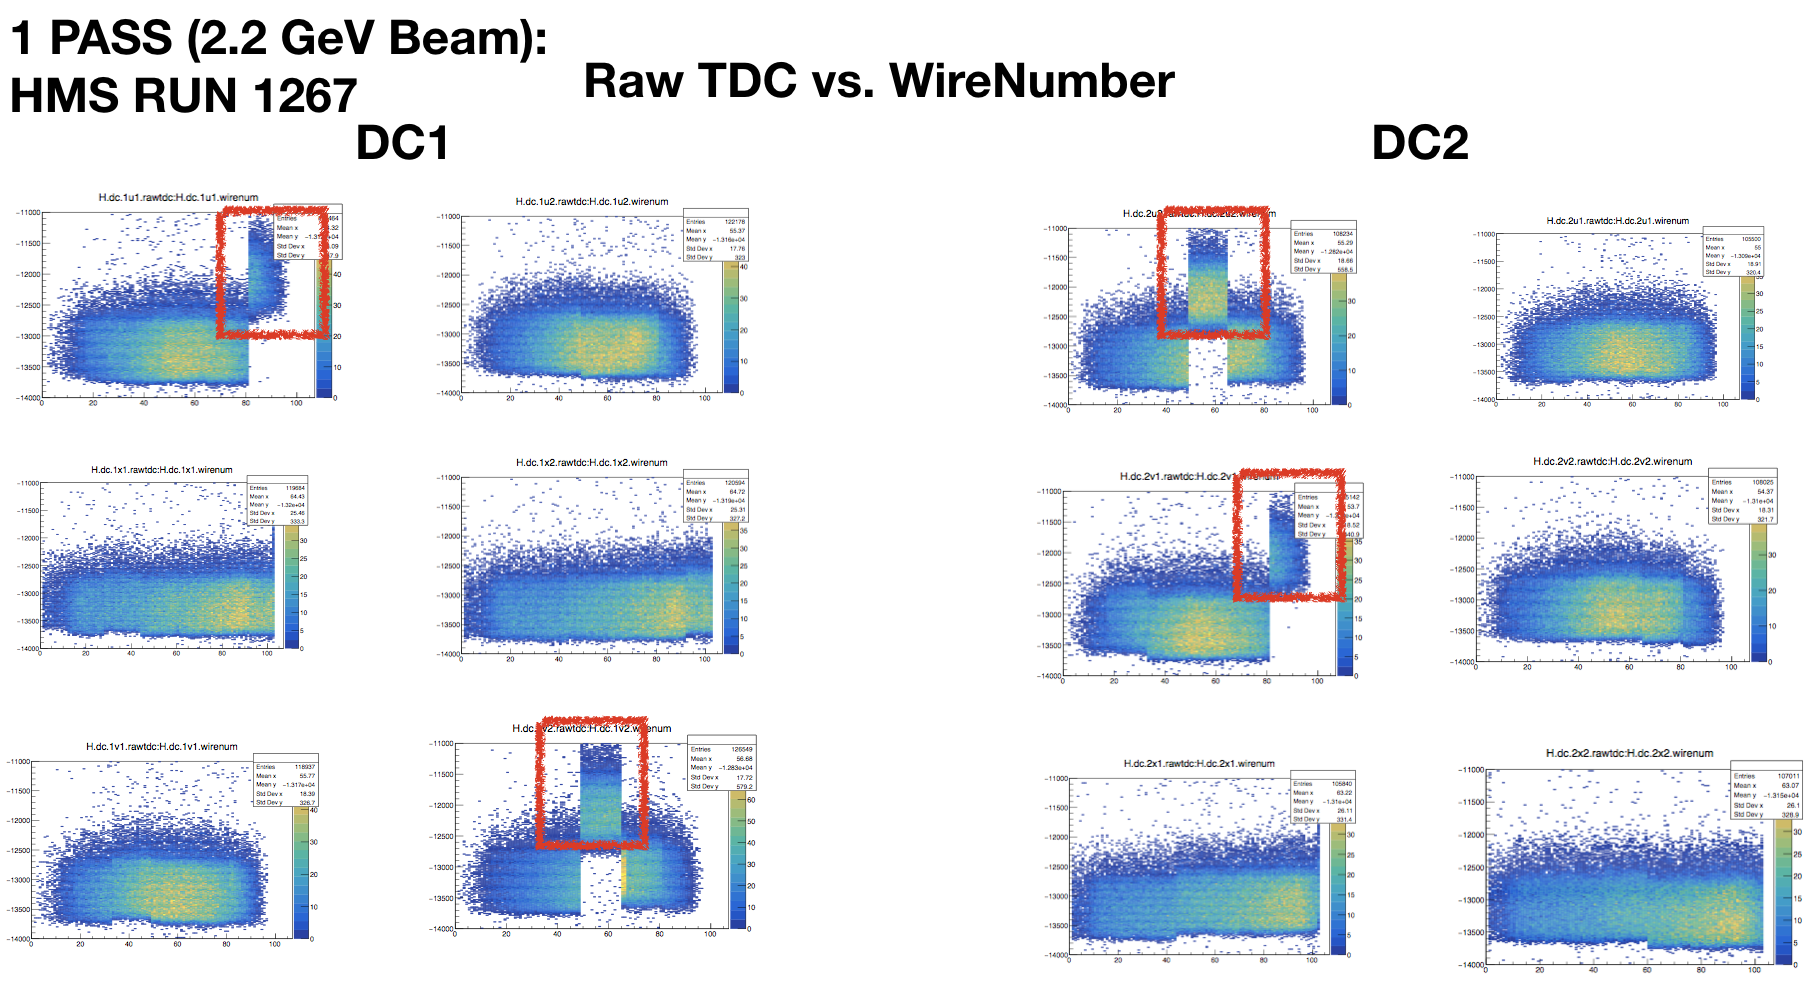
\includegraphics[width=6.0in, height=3.0in]{shifted_drifttimes.png}
  \caption{The Raw TDC vs. Wire Number Correlations for all 12 planes. An offset of $\sim$ 1000 Channels ($\sim$ 100 ns) is observed
    in wire groups of four distinct planes.}
  \label{fig:shift_dtimes}
\end{figure}
\newpage
In Figure \ref{fig:wire_residual}, the redisuals for the tracks are plotted as a function of wire number. It can be clearly observed that the same four groups mentioned in
Figure \ref{fig:shift_dtimes} have smeared out residuals. At this point, I started to consider this issue seriously, as it was NOT simply drifted times which could be fixed in
software, but now the tarcking had been affected.
\begin{figure}[h!]
  \centering
  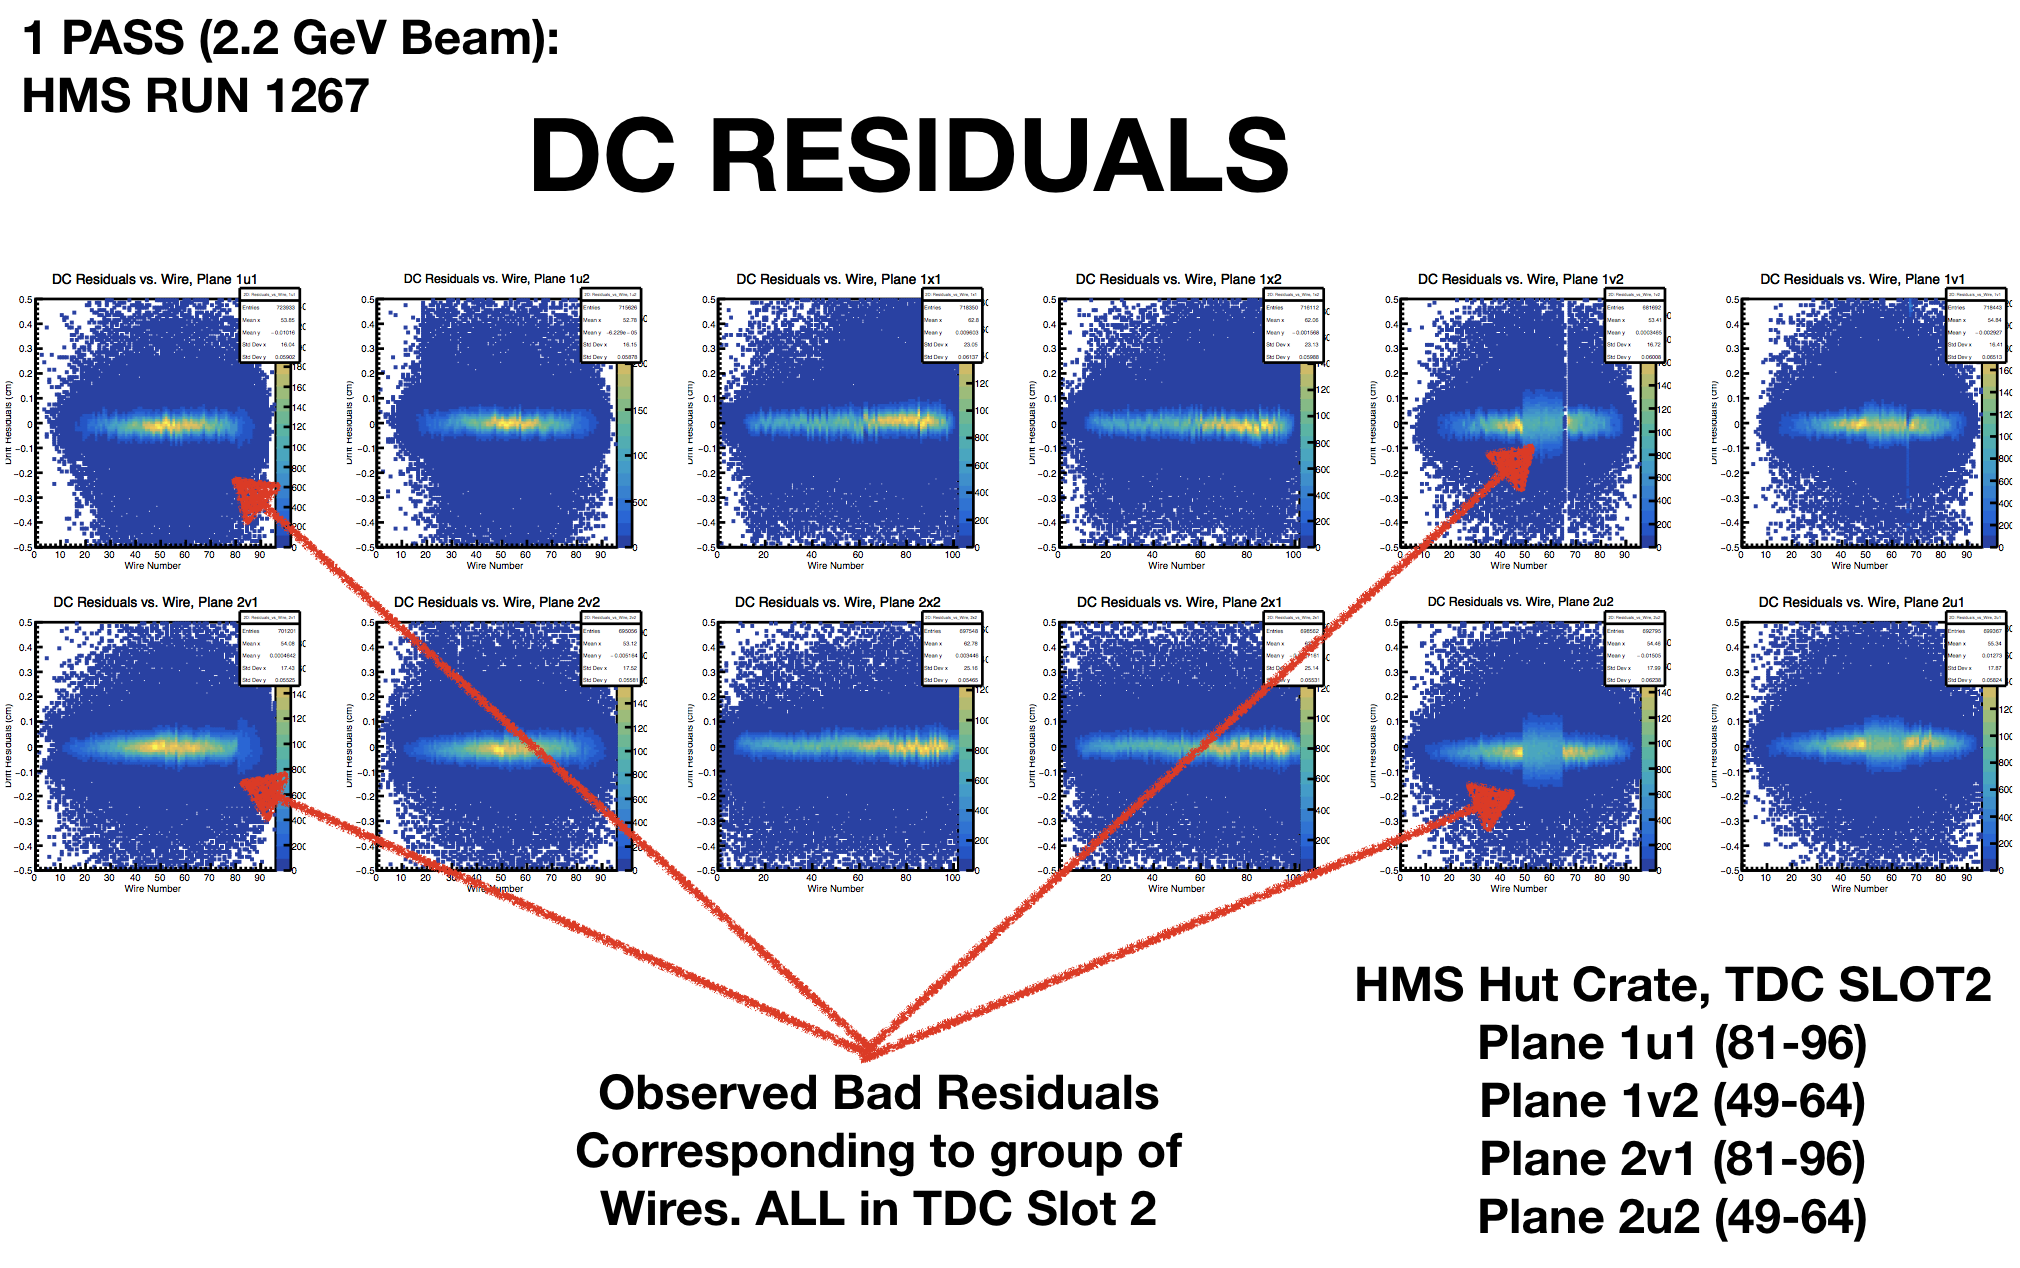
\includegraphics[width=7.0in, height=4.0in]{bad_wireresidual.png}
  \caption{Correlation of Residuals vs. Wire Number for all 12 planes. Four wire groups stand out from the rest, with a noticeable smearing.
  The adjacent planes are affected by this smearing as well, even though they are NOT part of the problematic TDC.}
  \label{fig:wire_residual}
\end{figure}
\begin{figure}[h!]
  \centering
  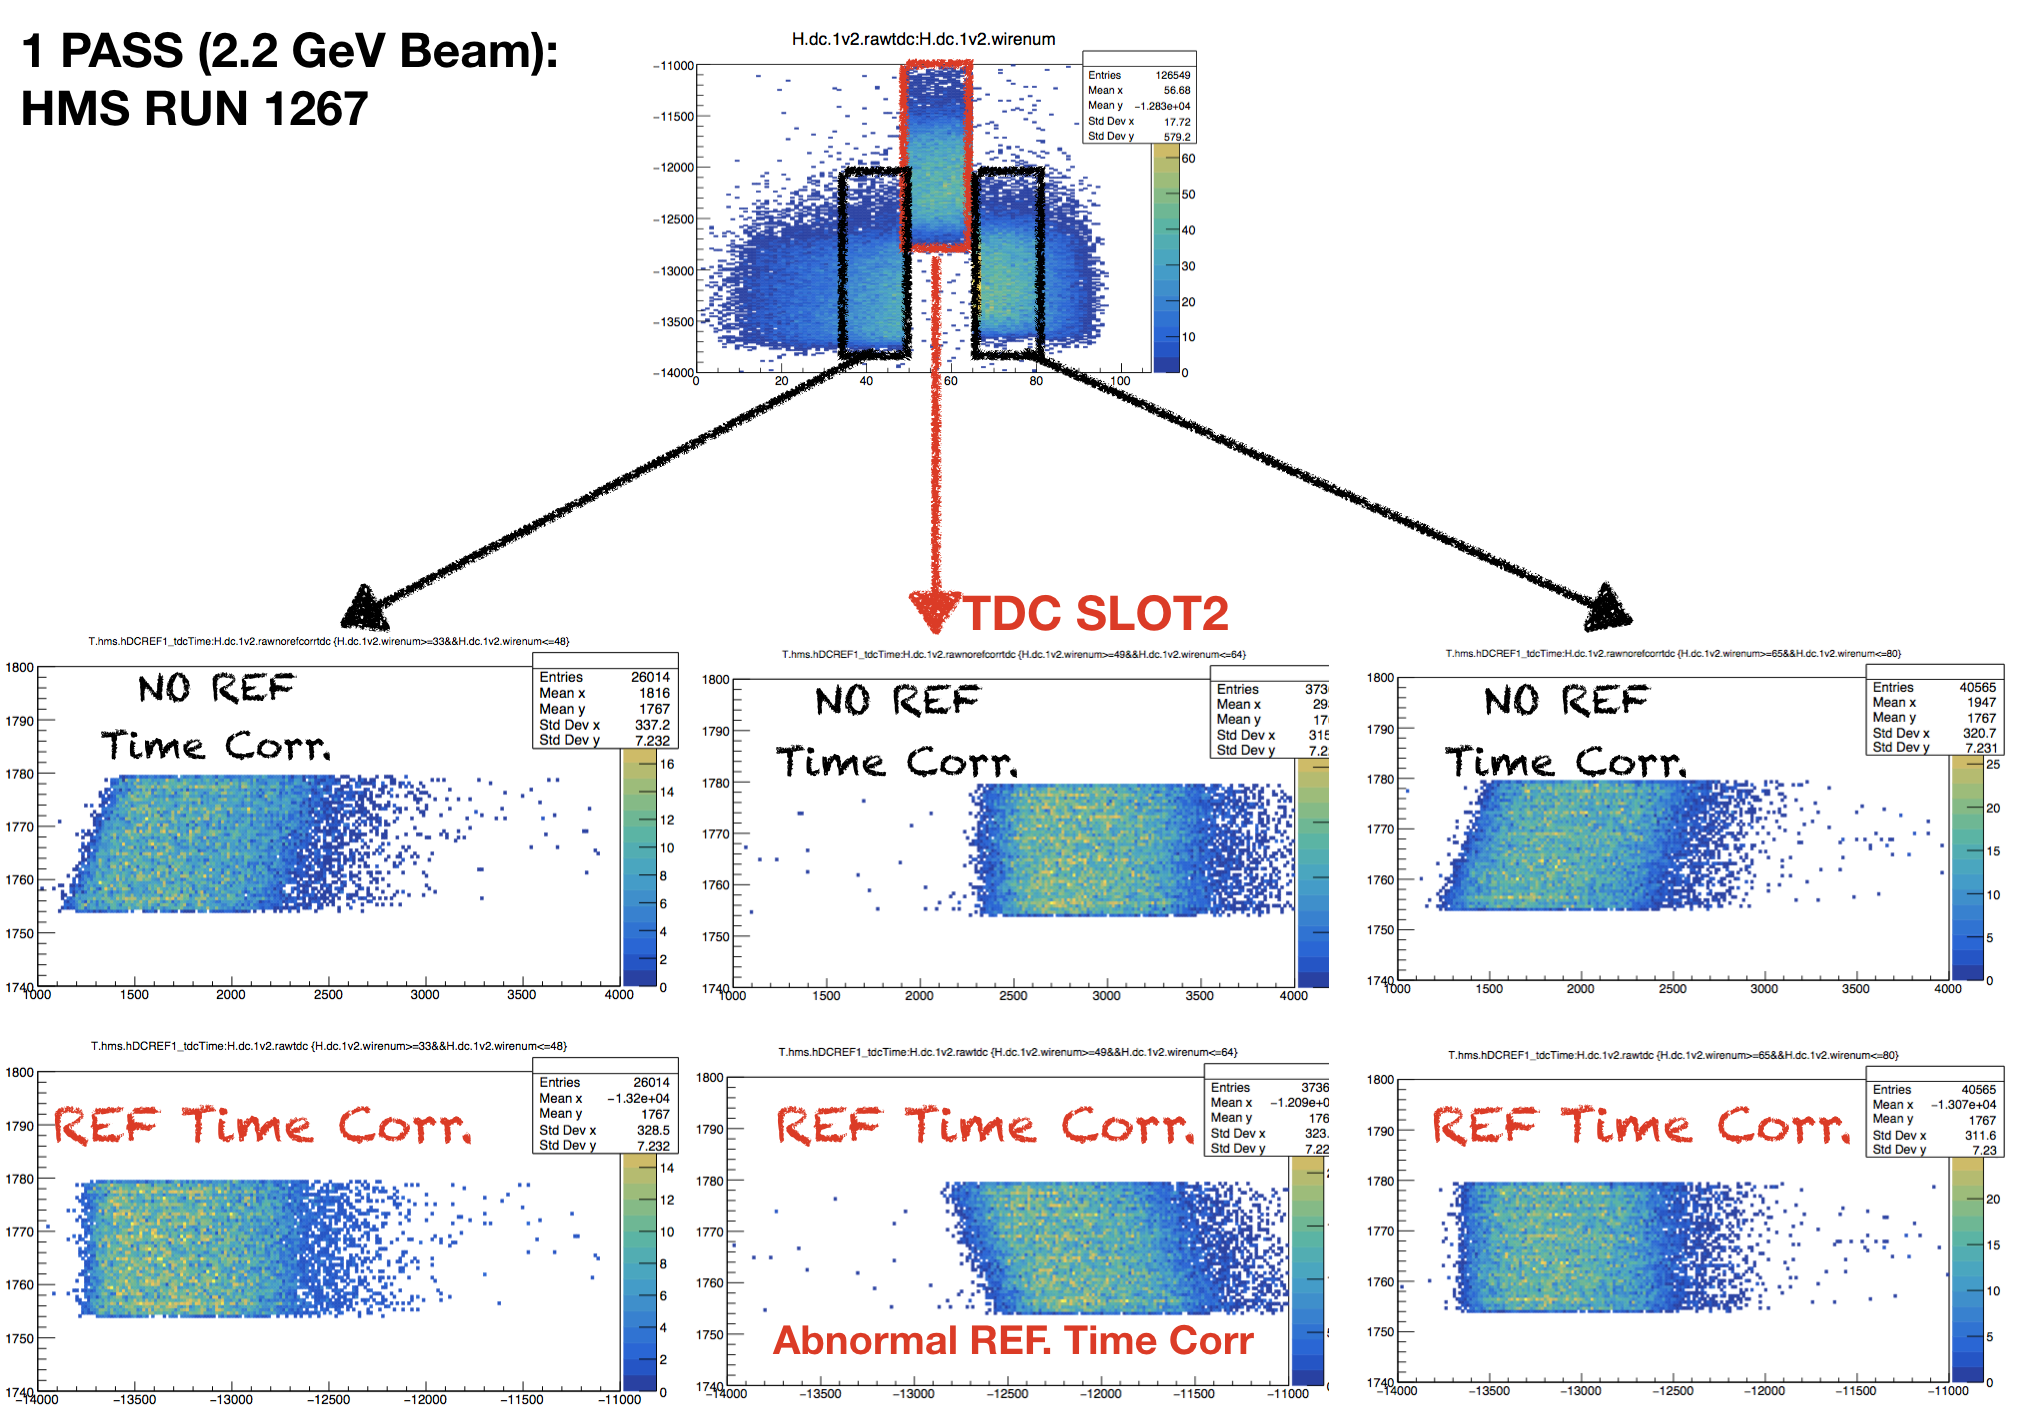
\includegraphics[width=5.1in, height=3.1in]{hDC_RefTime_correlation.png}
  \caption{Correlation between the HMS DC reference time and the raw TDC times. The DC 1, V'-Plane raw TDC vs. Wire Number is shown. Adjacent wirgroups which
    are NOT in TDC Slot 2 are compared to the TDC Slot 2 wire group before and after applying the reference time correction to the raw TDC time. The vertical axis
  is the HMS DC reference time corrected from itself (ns units). The horizontal axis is the raw TDC time in units of Channel ($\sim$0.1 ns/Channel).}
  \label{fig:hDC_correlation}
\end{figure}
\newpage
Figure \ref{fig:hDC_correlation} is determinant in this study, as it shows the correlation of the reference time with the raw TDC time before and after applying the reference time correction.
As expected from a normal TDC, when tdc times are reference time subtracted, the correlation dissappears. However, in TDC Slot 2, the reference time and raw tdc time
are uncorrelated, which is an indication that it is Out-of-Sync with the rest of the modules. When the raw TDC time for Slot 2 is corrected with the reference
time from another Slot, the corrected TDC time now has a correlation with the reference time which is indicative of a synchronization issue.
The reference time spans over a 25 ns range, even though it is reference time corrected from itself, which is due to the intrinsic 25 ns jitter coming from the TDC internal 40 MHz clock. The
raw TDC time spans over a $\sim$ 100 ns range, and at the smallest range, which corresponds to drift times of particles nearest to the sense wires, one can clearly see a
correlation with the reference time. 

\section{Temporary Solution for the Out-Of-Sync TDC}
\indent As a temporary solution (until we replace the TDC module), it was decided that a copy of the reference time should be fed independently to the bad TDC module. This way, the TDC can synchronize with its own
reference time, as opposed to receiving an alternate copy from the trigger interface (TI) module. This modification was done on hardware on July 30, 2018. See Log Enrty \url{https://logbooks.jlab.org/entry/3583094}.

\begin{figure}[h!]
\centering
\begin{subfigure}{.5\textwidth}
  \centering
  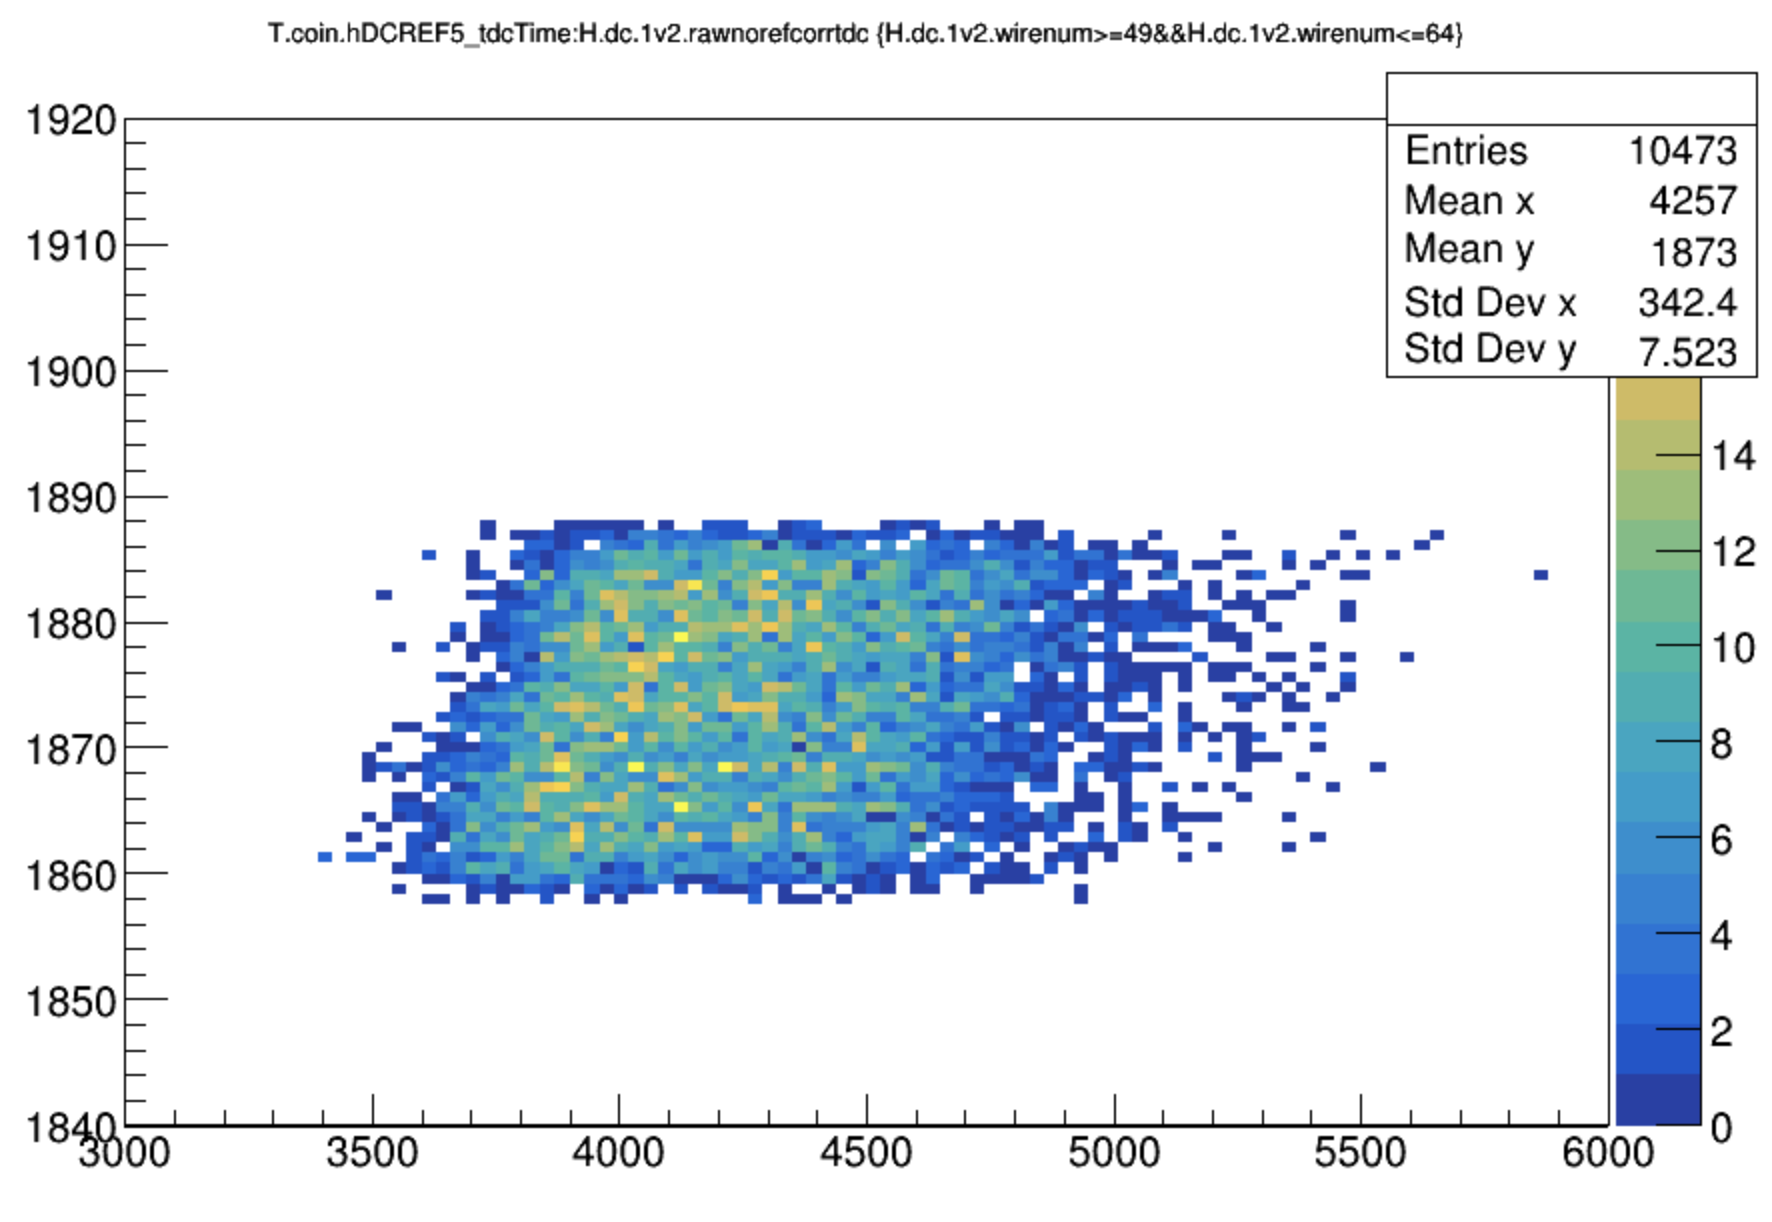
\includegraphics[width=.8\linewidth]{hdcref5_corr.png}
  \caption{TDC Slot 2 Reference Time vs. Raw Uncorrected TDC \\Time for wire group 1V2 (49-64)}
  \label{fig:ref5_correlated}
\end{subfigure}%
\begin{subfigure}{.5\textwidth}
  \centering
  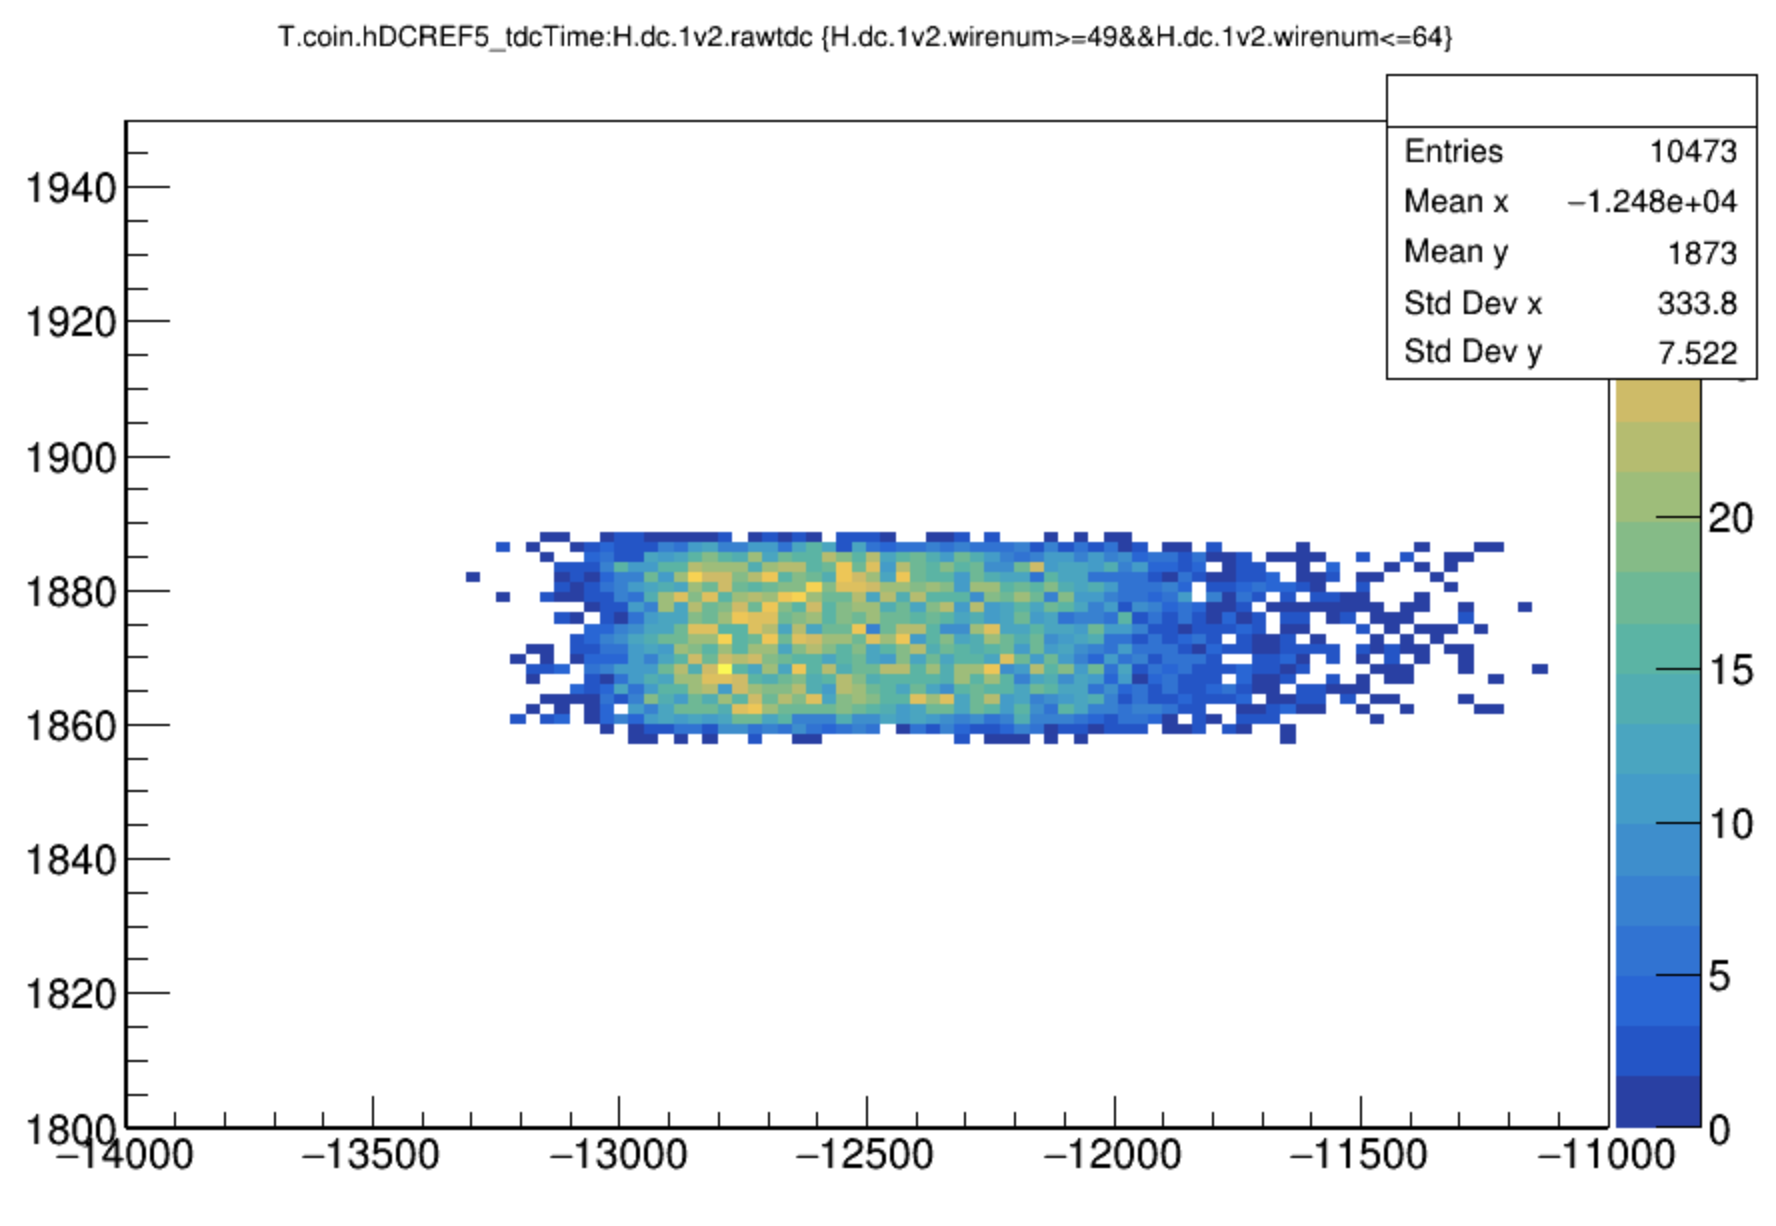
\includegraphics[width=.8\linewidth]{hdcref5_uncorr.png}
  \caption{TDC Slot 2 Reference Time vs. Raw Corrected TDC \\Time for wire group 1V2 (49-64)}
  \label{fig:ref5_uncorrelated}
\end{subfigure}
\caption{Results of HMS singles (DAQ in Coincidence Mode) cosmic run 4437 to verify that adding the new reference time to TDC Slot 2 fixes the problem.
  The subfigures above show the correlation between the newly added reference time and raw TDC Time from a group of wires in TDC Slot 2. As shown in subfigure (b), the correlation
  between the new reference time and raw TDC time is NOT present when the raw time is reference time corrected.}
\label{fig:hdc_Ref5}
\end{figure}
\noindent To demonstrate that the new reference time added fixed the issue, I decided to take an HMS singles (DAQ in Coincidence Mode) cosmic run to prove that when the
new reference time was subtracted from the raw TDC time, the correlation that was present originally, dissappeared. This was indeed what happened, as observed in Figure \ref{fig:hdc_Ref5}.\\
\indent A modification in software map was also necessary, as the TDC Slot 2 needed to point to the new reference time. This change affects the data replay from the
Spring 2018 Commissioning Run Period since during that time, TDC Slot 2 was pointing to a different reference time in the software. Therefore, if you have the most up-to-date copy of the
hallc replay analyzer, to replay data from the previous run period, make sure to load the correct map into the replay script being used. See Figure \ref{fig:map} 

\begin{figure}[h]
  \centering
  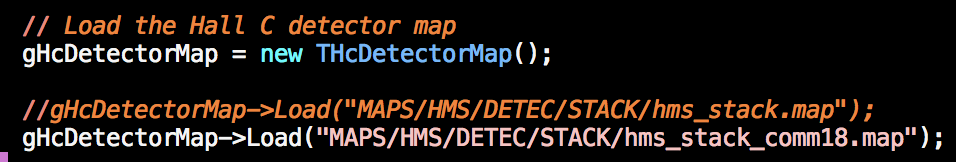
\includegraphics[width=5.0in, height=1.0in]{loadmap.png}
  \caption{Snippet of the hms replay script that shows how to load the correct map for Spring 2018 run period.}
  \label{fig:map}
\end{figure}
\newpage
\section{How to Minimize the impact the Out-of-Sync TDC had on Residuals }
\noindent The group of wires that were affected by the TDC synchronization issue cannot be restored to normal, so their residuals will remain significantly smeared out. Fortunately,
two of the groups are located at the edge of each chamber, so they have minimal impact. The other two groups, even though they are near the center of the chamber, they are
in different chambers, so tracking in NOT severely affected. The group of wires in adjacent planes are affected (See Figure \ref{fig:wire_residual}) by this smearing, since
they depend heavily on their adjacent partners (U,V planes) for the (x,y) coordinate determination from tracking. To minimize this effect, the Hall C source code \textit{hcana}
was modified to read in the sigma parameters on a per-wire basis, if a certain flag is set. Originally, the sigma parameters were read on a per-plane basis, and were assigned a
value of 0.02 by default. If the sigma-per-wire flag is set, then the sigma parameter values are read on a wire-by-wire basis, and the wire groups associated with the
Out-of-Sync TDC are assigned a sigma of 0.06, while the rest are assigne a value of 0.02 so that during the track-fitting algorithm, if a track passes though one of this groups,
they will have a smaller contribution (or weight) to the fit. The results are shown in Figures \ref{fig:wire_residuals_flag}.
\begin{figure}[h!]
\centering
\begin{subfigure}{.5\textwidth}
  \hspace*{-5cm}                                                           
  \centering
  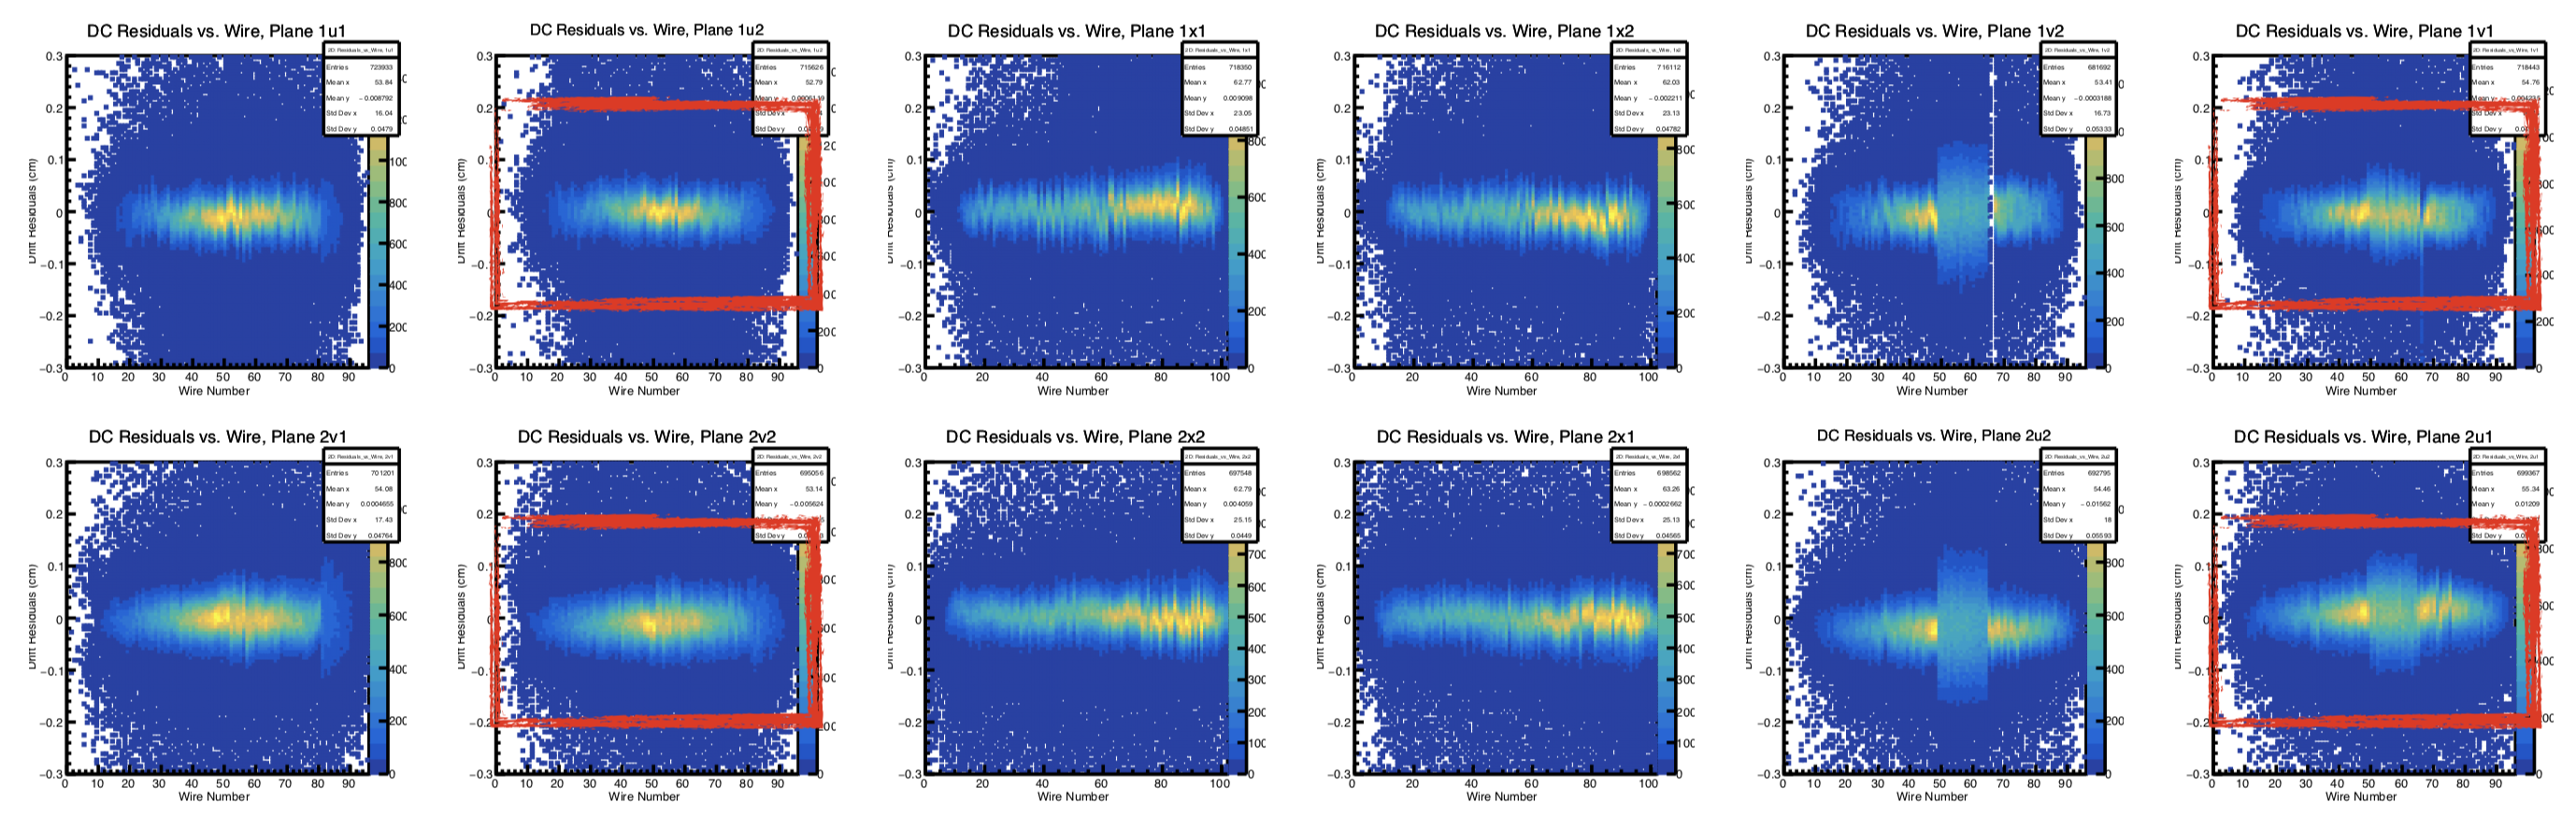
\includegraphics[width=2.1\linewidth]{2d_residuals_flagOFF.png}
  \subcaption{Residuals vs. Wire Number for all Chamber planes, with sigma-per-wire flag \textit{OFF}.}
  \label{fig:2d_res_flagOff}
\end{subfigure}%

\begin{subfigure}{.5\textwidth}
\hspace*{-5cm}                                                           
  \centering
  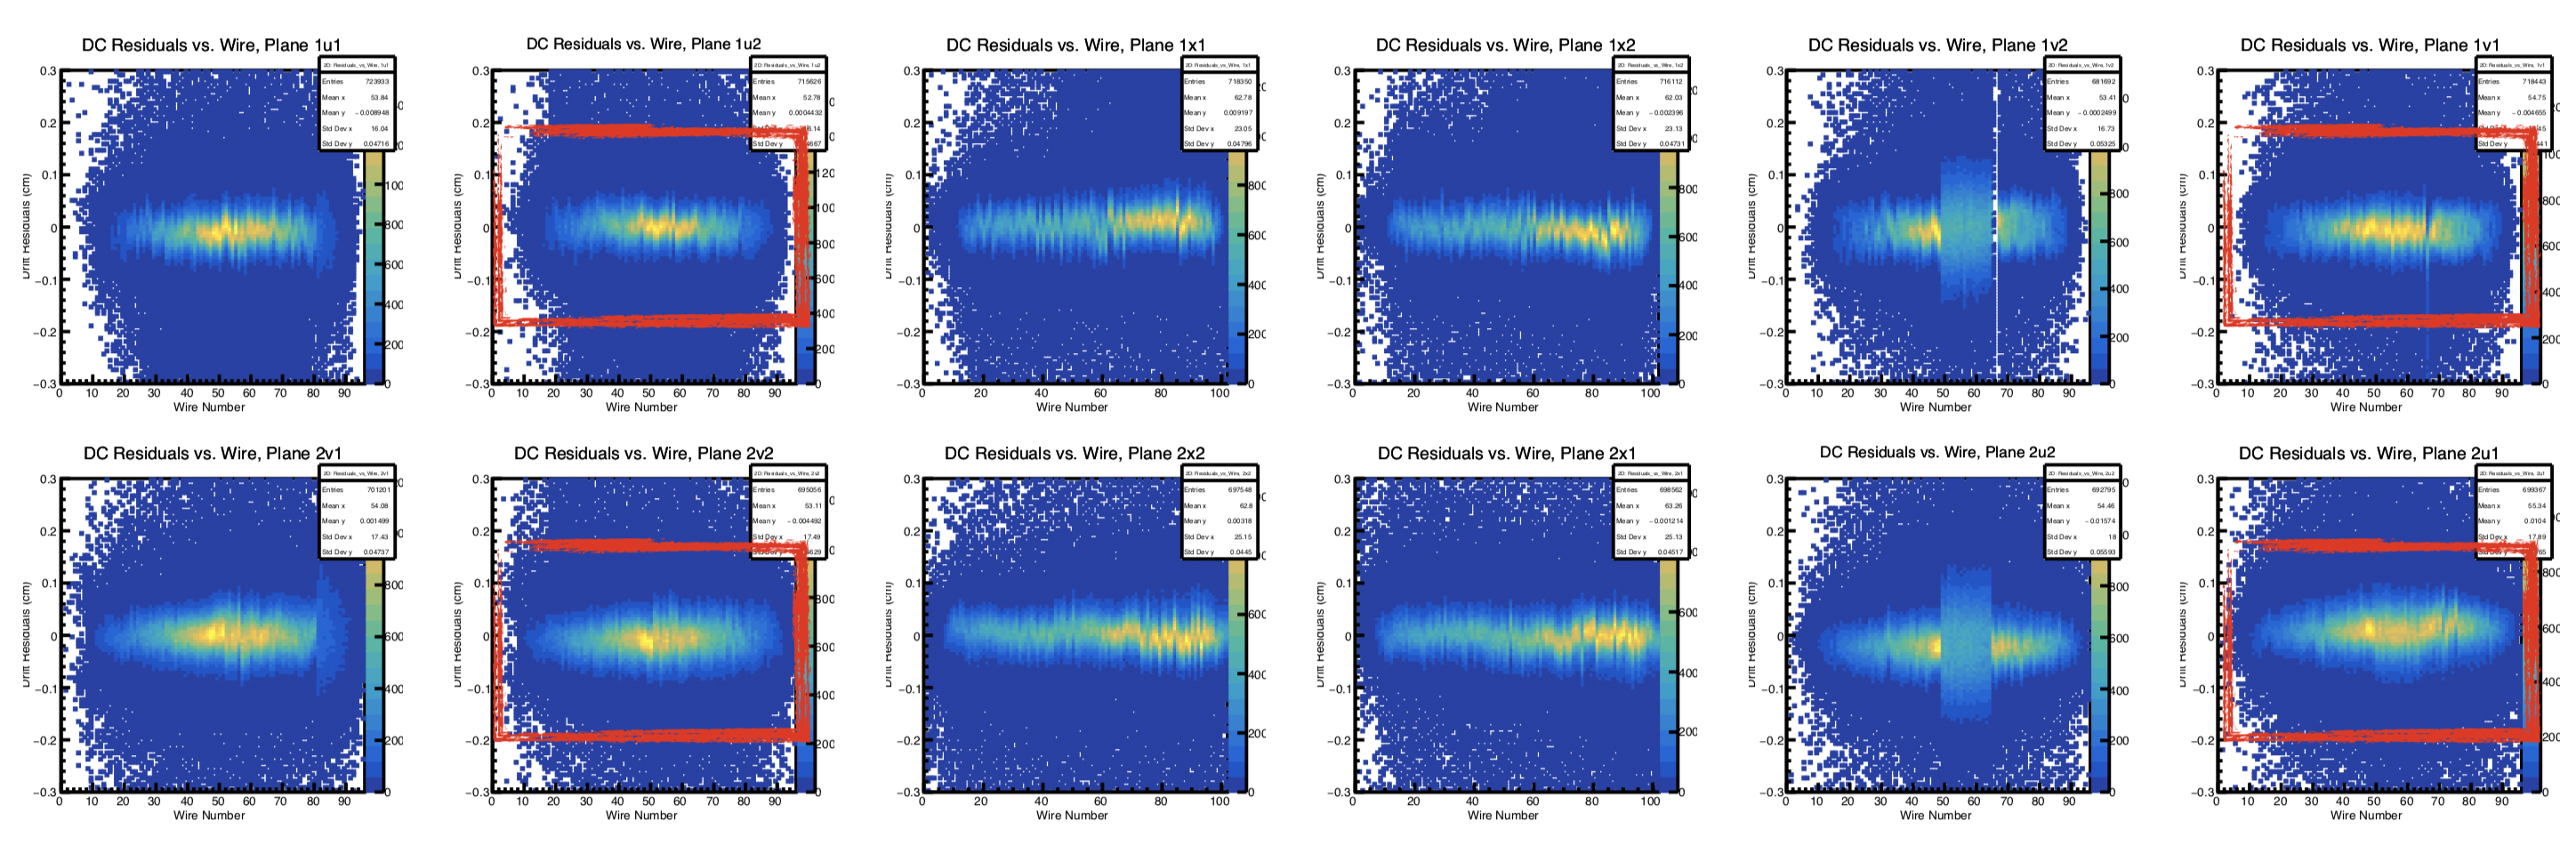
\includegraphics[width=2.1\linewidth]{2d_residuals_flagON.png}
  \caption{Residuals vs. Wire Number for all Chamber planes, with sigma-per-wire flag \textit{ON}.}
  \label{fig:2d_res_flagON}
\end{subfigure}
\caption{Residuals vs. Wire Number for all Chamber planes. The \textcolor{red}{RED BOXES} highlight the group of wires that were affected, but had nothing to do with the
  out-of-sync TDCs wire groups.}
\label{fig:wire_residuals_flag}
\end{figure}\\
In subfigure (b), when a sigma of 0.06 was applied to the bad groups (Planes 1u1, 1v2, 2v1, 2u2), the adjacent planes (highlighted in \textcolor{red}{RED})
wire residuals improved significantly. This is due the fact that less weight (larger sigma($\sigma$)) was given to the affected group of wires.
To quantify by how much the group residuals highlighted in Figure \ref{fig:wire_residuals_flag} have improved, I plotted the 1D-projection of such wire groups.
There seemed to be a noticable improvement with up to $\sim$ 60 $\mu$m in the residuals. See Figure \ref{fig:group_residuals} below.
\begin{figure}[ht!]
  \centering
  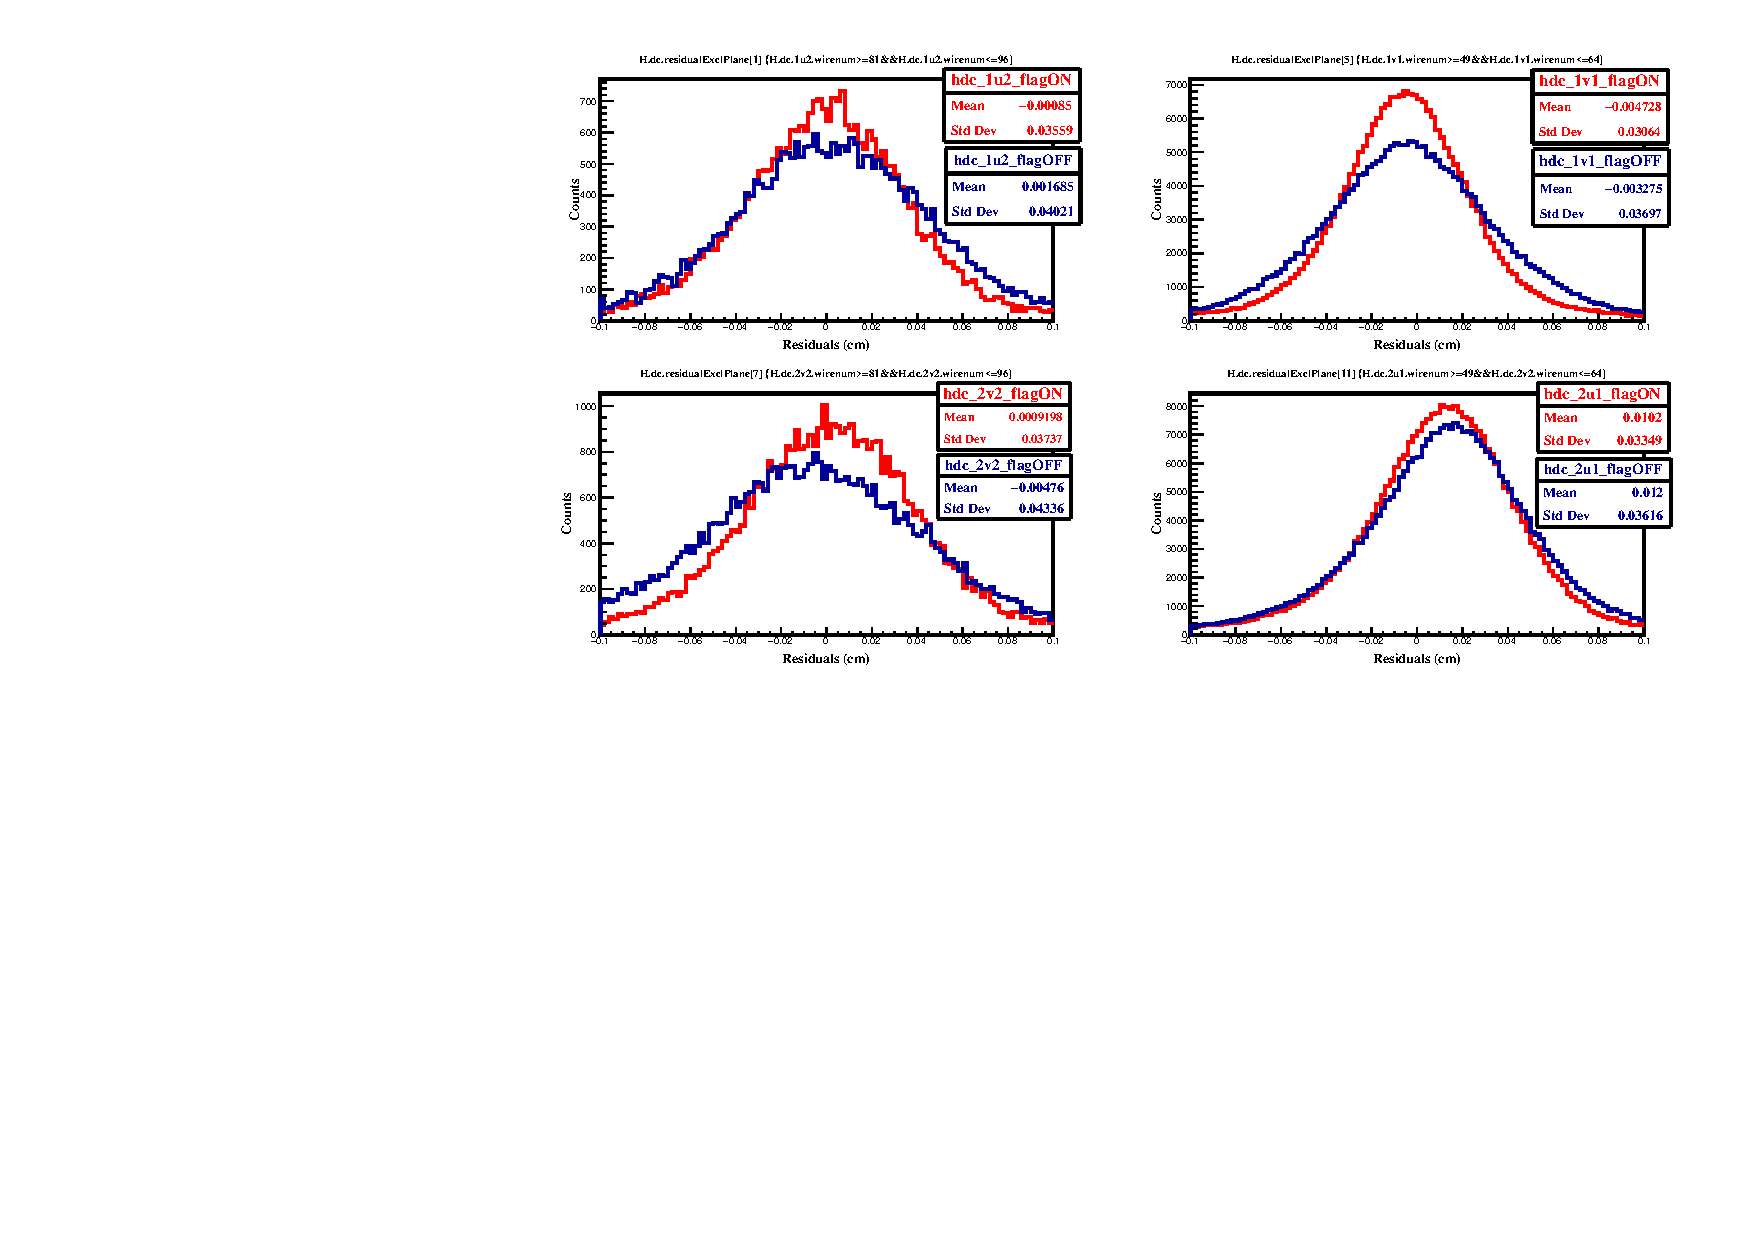
\includegraphics[width=7.0in, height=4.0in]{group_residuals.pdf}
  \caption{Residuals of highlighted wire groups in Figure \ref{fig:wire_residuals_flag}}
  \label{fig:group_residuals}
\end{figure}\\
The plane residuals, however, did not have much improvement after increasing the weight factor. At most, there was a 25 $\mu$m improvevent in the Standard Deviation.
See Figure \ref{fig:plane_residuals}
\begin{figure}[ht!]                                                          
%  \vspace*{10.5cm}                                                           
  \centering
  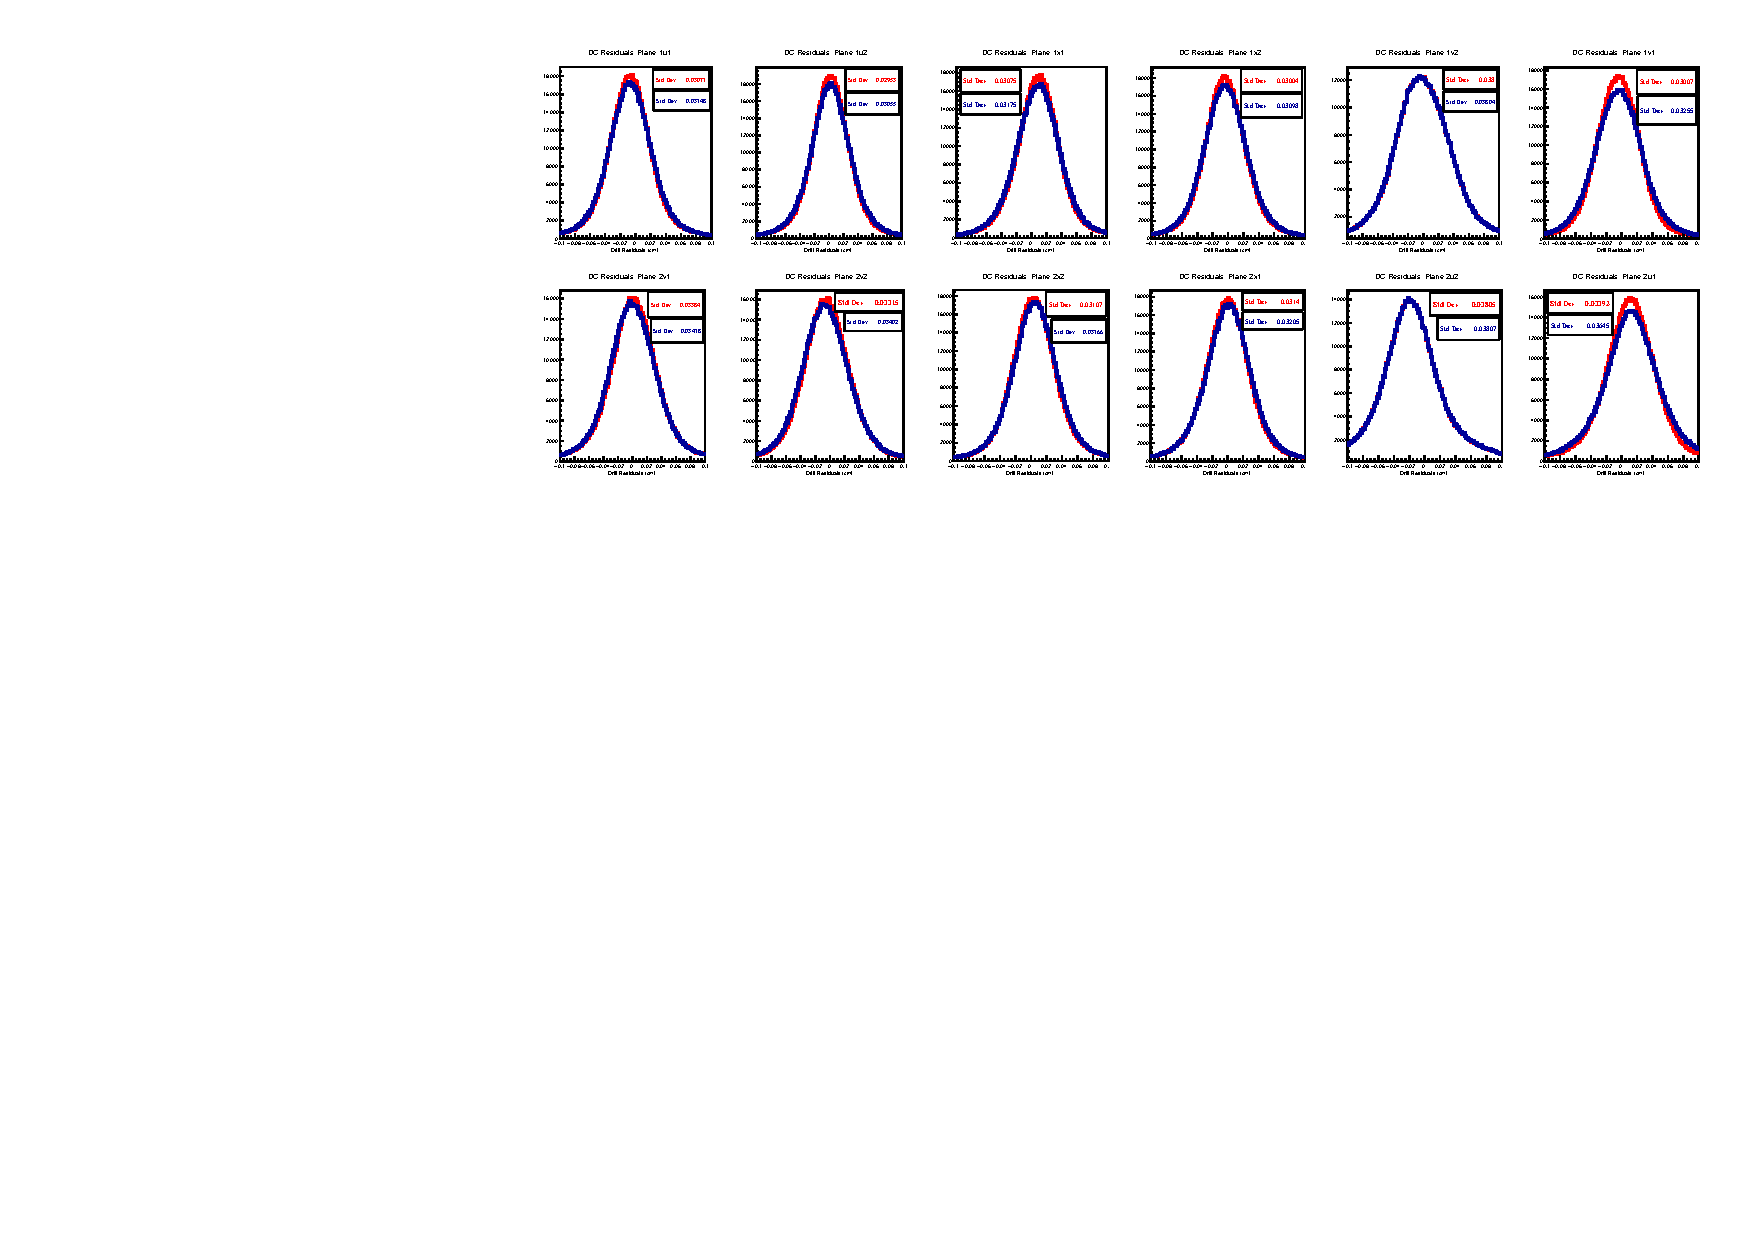
\includegraphics[width=7.5in, height=3.0in]{residuals_compare.pdf}
  \caption{Plane residuals with the sigma-per-wire flag ON (\textcolor{red}{RED}) and OFF (\textcolor{navyblue}{BLUE})}
  \label{fig:plane_residuals}
\end{figure}
\newpage
\noindent It is importnant to note that the sigma-per-wire flag and the parameter file are NOT included in \texttt{hallc$\_$replay}, since this is a very specific scenario that
ONLY applies to the Winter-2017/Spring-2018 Run Period. If users who took data during that time, and would like to try adding this flag and the parameter file,
the instructions are as follows:
\begin{itemize}
\item  Create the parameter file in path: \texttt{/PARAM/HMS/DC/hdc$\_$sigma$\_$per$\_$wire.param} \par
  \begin{minipage}{\linewidth}
    \centering
    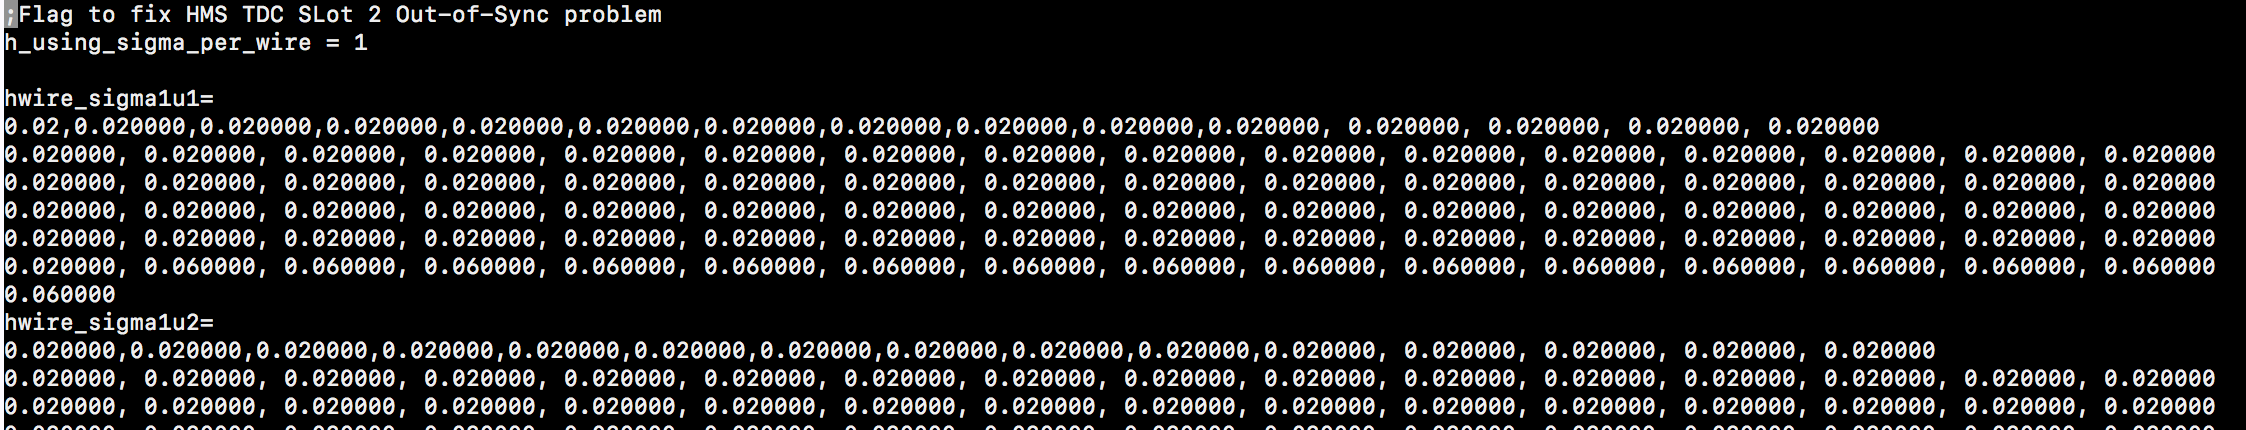
\includegraphics[width=15cm]{param.png}
    \captionof{figure}{Snippet of sigma-per-wire parameter file.}
    \label{fig:param}
  \end{minipage}
\item  Include the parameter file in path: \texttt{/DBASE/HMS/general.param} \par
  \begin{minipage}{\linewidth}                                                          
    \centering
    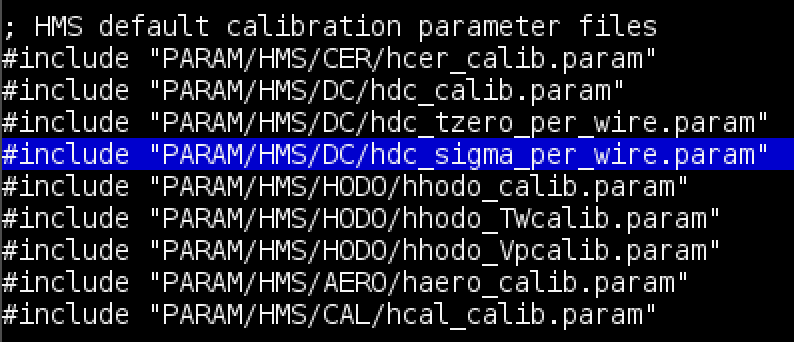
\includegraphics[width=10cm]{gen_parm.png}
    \captionof{figure}{Snippet of general.param file.}
    \label{fig:gen_param}
  \end{minipage}
\end{itemize}
\noindent In case you need help or do NOT have the time to create this parameter file, I have uploaded both the script that produces the parameter file and the parameter file
itself to my github page. \\
\textbf{Link to script:} \\ \url{https://github.com/Yero1990/scientific_articles/blob/master/Spring_2018_Run/OutOfSync_TDC/write_sig_param.C} \\
\textbf{Link to parameter file:} \\\url{https://github.com/Yero1990/scientific_articles/blob/master/Spring_2018_Run/OutOfSync_TDC/hdc_sigma_per_wire.param}

\newpage
\onecolumn
\bibliography{template}
\bibliographystyle{acm}


\end{document}
